\begin{verbatim}
\subsection{Sine functions}
For given $x \in [0, 2\pi]$ with step size $\pi/12$, we can obtain the
evaluations of \eqref{eq:y1}, \eqref{eq:y2}, \eqref{eq:y3} at $x$
(see Table \ref{tab:sin}), and the corresponding plot (see Figure \ref{fig:sin}).
\begin{align}
y_1 & = \sin(x/2) \label{eq:y1}
y_2 & = \sin(x)   \label{eq:y2}
y_3 & = \sin(2x)  \label{eq:y3}
\end{align}
\begin{table}[!hbtp]
\centering
\caption{Sine functions}
\label{tab:sine}
\begin{tabular}{lcrr}
\toprule
        $x$ & $\sin(x/2)$ &   $\sin(x)$ &  $\sin(2x)$ \\
\midrule
$ 0.000000$ & $ 0.000000$ & $ 0.000000$ & $ 0.000000$ \\
$ 0.261799$ & $ 0.130526$ & $ 0.258819$ & $ 0.500000$ \\
$ 0.523599$ & $ 0.258819$ & $ 0.500000$ & $ 0.866025$ \\
$ 0.785398$ & $ 0.382683$ & $ 0.707107$ & $ 1.000000$ \\
$ 1.047198$ & $ 0.500000$ & $ 0.866025$ & $ 0.866025$ \\
$ 1.308997$ & $ 0.608761$ & $ 0.965926$ & $ 0.500000$ \\
$ 1.570796$ & $ 0.707107$ & $ 1.000000$ & $ 0.000000$ \\
$ 1.832596$ & $ 0.793353$ & $ 0.965926$ & $-0.500000$ \\
$ 2.094395$ & $ 0.866025$ & $ 0.866025$ & $-0.866025$ \\
$ 2.356194$ & $ 0.923880$ & $ 0.707107$ & $-1.000000$ \\
$ 2.617994$ & $ 0.965926$ & $ 0.500000$ & $-0.866025$ \\
$ 2.879793$ & $ 0.991445$ & $ 0.258819$ & $-0.500000$ \\
$ 3.141593$ & $ 1.000000$ & $ 0.000000$ & $-0.000000$ \\
$ 3.403392$ & $ 0.991445$ & $-0.258819$ & $ 0.500000$ \\
$ 3.665191$ & $ 0.965926$ & $-0.500000$ & $ 0.866025$ \\
$ 3.926991$ & $ 0.923880$ & $-0.707107$ & $ 1.000000$ \\
$ 4.188790$ & $ 0.866025$ & $-0.866025$ & $ 0.866025$ \\
$ 4.450590$ & $ 0.793353$ & $-0.965926$ & $ 0.500000$ \\
$ 4.712389$ & $ 0.707107$ & $-1.000000$ & $ 0.000000$ \\
$ 4.974188$ & $ 0.608761$ & $-0.965926$ & $-0.500000$ \\
$ 5.235988$ & $ 0.500000$ & $-0.866025$ & $-0.866025$ \\
$ 5.497787$ & $ 0.382683$ & $-0.707107$ & $-1.000000$ \\
$ 5.759587$ & $ 0.258819$ & $-0.500000$ & $-0.866025$ \\
$ 6.021386$ & $ 0.130526$ & $-0.258819$ & $-0.500000$ \\
$ 6.283185$ & $ 0.000000$ & $-0.000000$ & $-0.000000$ \\
\bottomrule
\end{tabular}
\end{table}

\begin{figure}[!hbtp]
    \centering
    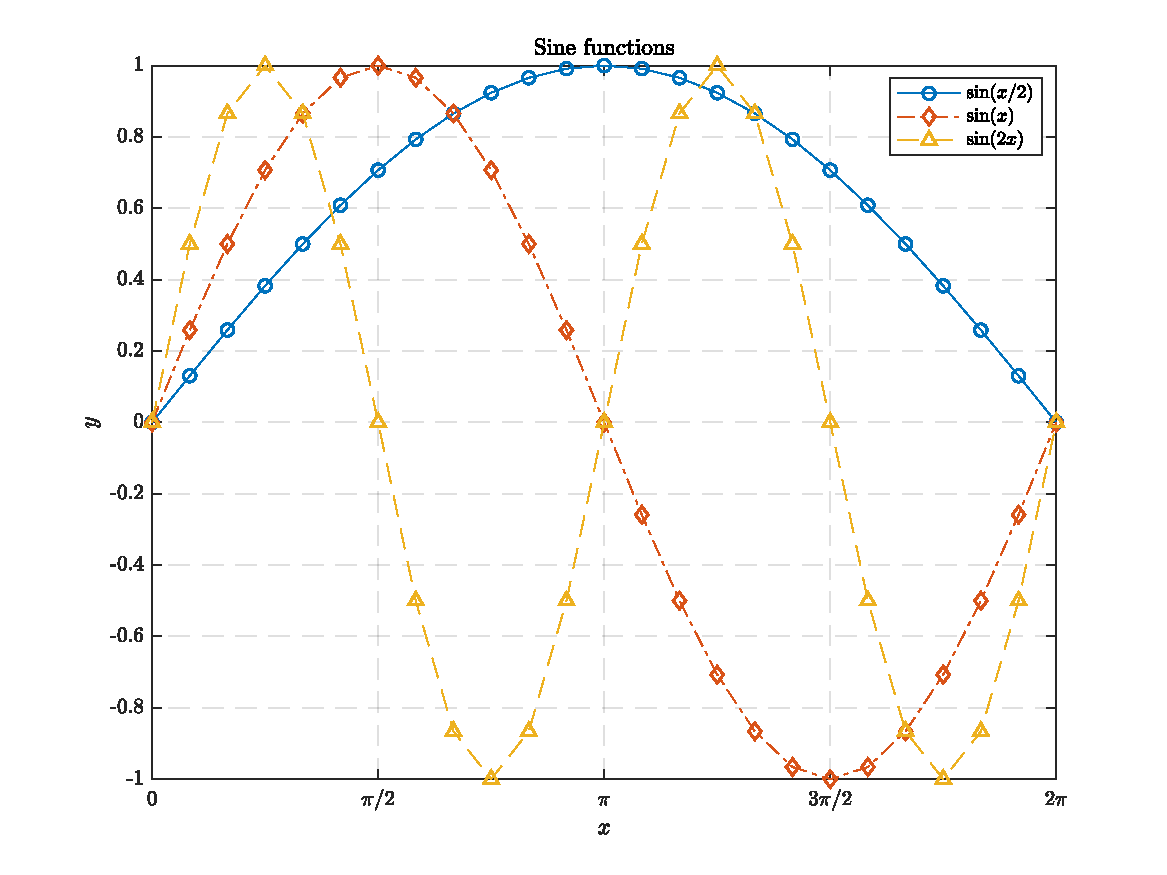
\includegraphics[width=0.75\textwidth]{../src/lab_05_plot.pdf}
    \caption{Sine functions}
    \label{fig:sin}
\end{figure}
\end{verbatim}
